
\section{Bitwise operaties.}
\label{chap:biw}

Zoals in hoofdstuk \ref{sec:matrix} staat vermeldt heeft de firma Adafruit voor het matrix display een speciale component gemaakt waardoor het matrix display eenvoudig te programmeren is. Listing \ref{lst:matrixaan} is hier een voorbeeld van.
\begin{lstlisting}[caption={Het aanzetten van een LED},label={lst:matrixaan}]
#include <Adafruit_Microbit.h>
#define LED0 0  //definieer LEDx tot een waarde
#define LED1 1
#define LED2 2
#define LED3 3
#define LED4 4

Adafruit_Microbit_Matrix matrixMbit; //maak een LED matrix aan.
const uint8_t
smile_bmp[] =
{ B00000,
	B01010,
	B00000,
	B10001,
	B01110, };
uint8_t matrixje[] =
{ B00000,
	B00000,
	B00000,
	B00000,
	B00000, };

void setup() {
	Serial.begin(9600);
	Serial.println("Welkom bij embedded!");
	
	matrixMbit.begin();
	matrixMbit.show(smile_bmp);
	delay(2000);
	matrixMbit.show(matrixje);
	delay(2000);  
	//zet rechterLED bovenste rij aan
	matrixje[0]= 1 << LED0; //schuif 1, LED0 plaatsen op naar links.
	matrixMbit.show(matrixje);
	delay(2000);  
	//zet linkerLED bovenste rij aan 
	matrixje[0] = 1 << LED4; //schuif 1, LED4 plaatsen op naar links.
	matrixMbit.show(matrixje);
}
void loop() {
}
\end{lstlisting}
Wat opvalt aan Listing \ref{lst:matrixaan} is dat er een hoop define's staan aan het begin. De bedoeling van deze define's is dat de code eenvoudiger te lezen is.
Indien in de code  \small{\texttt{\textit{1 \textless\textless  ~LED4}}} staat, weet de lezer gelijk dat de $4^{e}$ LED bedoeld wordt. Verder is te zien hoe een LED aangezet kan worden door de betreffende bit in een array van 8 bits data, een 1 te maken. Dit wordt gedaan door een 1 (0b00000001) een aantal plaatsen naar links op te laten schuiven. Zoals te zien is in onderstaand statement:\\
\texttt{\textit{matrixje[0]= 1 \textless\textless  ~LED0;}}\\
Hierbij staat de \texttt{1} voor het aantal plaatsen dat LED0 naar links wordt opgeschoven. LED0 staat gedefinieerd op regel 2 van Listing \ref{lst:matrixaan}
\begin{enumerate}
	\item Installeer \href{https://learn.adafruit.com/use-micro-bit-with-arduino/adafruit-libraries}{de Adafruit Libraries} indien dit nog niet gedaan is.
	\item
	\begin{enumerate}

	\item Open voorbeeldcode matrixSmpl (dit is Listing \ref{lst:matrixaan}). 
	\item Breid het programma zodanig zodat uit, zodat zowel LED0 als LED4 van de 2e rij aangaan. Maak hierbij gebruik van de operatoren '\textless\textless' en '\textbar'(bitwise or). Doe dit zoals in de theorie besproken is.
	
%	\begin{table}[h!]
\setlength\arrayrulewidth{2pt}
		\begin{tabular}{|c|c|c|}
			\hline
%			\colorbox{yellow}{\textbf{A}} &\colorbox{yellow}{\textbf{B} & \colorbox{Yellow}{\textbf{AB}}   \\ \hline
          \rowcolor{yellow}
		    A  & B     & A \textbar~ B       \\ \hline          
		    0  & 0     & 0       \\ \hline
			0      & 1     & 1       \\ \hline
			1     & 0     & 1       \\ \hline
			1    & 1     & 1       \\ \hline
		\end{tabular}\\
De bitwise OR 
%	\end{table}
	
	\item Breid het programma uit zodat 2 seconde nadat beide LEDS uit B aangegaan zijn, de linker boven LED (LED4) weer uitgaat. Maak hierbij gebruik van de operatoren '\textless\textless' ,  '\&' en  ' $\sim$'. Doe dit zoals in de theorie besproken is.
	
	\setlength\arrayrulewidth{2pt}
	\begin{tabular}{|c|c|c|}
		\hline
		%			\colorbox{yellow}{\textbf{A}} &\colorbox{yellow}{\textbf{B} & \colorbox{Yellow}{\textbf{AB}}   \\ \hline
		\rowcolor{yellow}
		A  & B     & A \& B       \\ \hline          
		0  & 0     & 0       \\ \hline
		0      & 1     & 0       \\ \hline
		1     & 0     & 0       \\ \hline
		1    & 1     & 1       \\ \hline
	\end{tabular}\\
	De bitwise AND 
	\item Door met bitwise operaties te werken, kan op een eenvoudige wijze een LED dat aan is, uitgezet worden en een LED dat uit is aangezet worden. Dit kan gedaan worden met de exclusief OR operator, zoals te zien is in onderstaand tabel. 
	Breid het programma uit zodat 2 LEDS van de onderste rij aan en uitgaan door de exclusief OR functie te gebruiken. Maak hierbij onder ander gebruik van de operator \^ ~. Do dit zoals in de theorie besproken is.
	
	\setlength\arrayrulewidth{2pt}
	\begin{tabular}{|c|c|c|}
		\hline
		%			\colorbox{yellow}{\textbf{A}} &\colorbox{yellow}{\textbf{B} & \colorbox{Yellow}{\textbf{AB}}   \\ \hline
		\rowcolor{yellow}
		A  & B     & A \^ ~ B       \\ \hline          
		0  & 0     & 0       \\ \hline
		0      & 1     & 1       \\ \hline
		1     & 0     & 1      \\ \hline
		1    & 1     & 0       \\ \hline
	\end{tabular}\\
	De bitwise XOR 
	
	\item Er kan ook getest worden of een LED aan is met behulp van bitwise operatoren.\\	\textcolor{cyan}{uint8\_t} hulpje= matrixje[0];\\
	\textcolor{OliveGreen}{if}(hulpje ...  .....) \{ \\
\}.

Vul het \textcolor{arduinoGreen}{if} statement in en toon aan dat een LED aan of uit is.
 \end{enumerate}

\item In het volgende voorbeeld gaat steeds een LED van rechts naar links aan.

\begin{lstlisting}[caption={Looplicht van de bovenste rij.},label={lst:matrixaan2}]
#include <Adafruit_Microbit.h>

Adafruit_Microbit_Matrix matrixMbit; //maak een LED matrix aan.

uint8_t matrixje[] =
{ B00000,
	B00000,
	B00000,
	B00000,
	B00000, };

void setup() {
	Serial.begin(9600);
	Serial.println("Welkom bij embedded!");

    matrixMbit.begin();
	matrixMbit.show(matrixje);
	delay(1000);  
}

uint8_t nr=0;
uint8_t hulpje;

void loop() {
	hulpje = 1 << nr; //schuif 1, nr plaatsen op naar links.
	matrixje[0]=hulpje; //De bovenste rij van de matrix krijgt de 
	matrixMbit.show(matrixje);
	delay(1000);
	nr++;
	if (nr == 5) {
	    nr=0;
	}        
}
\end{lstlisting}
Op regel 5 wordt een matrix component aangemaakt. Het tonen van de matrix wordt met de show functie gedaan (regel 16 en en 26).

\begin{enumerate}
	\item Download de  \href{https://github.com/JohnVi-hhs/embsysP/tree/main/voorbeelden/matrixloopl.ino}{voorbeeldcode van GitHub} of van brightspace of kopieer listing \ref{lst:matrixaan} in een nieuwe Arduino schets en voer deze uit.\\
	Probeer de uitvoer te verklaren.

\item Maak een functie \texttt{void \textit{zetLedAan}(unint8\_t rij,uint8\_t kolom);} die de LED op kolom en rij aanzet. Maak hierbij gebruik van de bitwise operator \textbar ~ zoals besproken tijdens de les.
\item Maak een functie \texttt{void \textit{zetLedUit}(unint8\_t rij,uint8\_t kolom);} die de LED op kolom en rij uitzet. Maak hierbij gebruik van de bitwise operatoren \& en $\sim$ zoals besproken tijdens de les.
\item Maak een functie \texttt{bool \textit{isLedAan}(unint8\_t rij,uint8\_t kolom);} die checkt of de LED op kolom en rij aan is. Maak hierbij gebruik van een bitmasker zoals besproken tijdens de les.

	\item Pas listing \ref{lst:matrixaan} met behulp van de bovenstaande functies zodanig aan, zodat:
\begin{enumerate}%[label=\arabic*.]
	\item Nadat de eerste rij geweest is, bij de tweede rij de ledjes \'{e}\'{e}n voor \'{e}\'{e}n  aangaan. 
	\item Na de tweede rij bij de derde rij de ledjes \'{e}\'{e}n voor \'{e}\'{e}n  aan gaan. 
	\item Na de laatste rij bij de eerste rij de ledjes \'{e}\'{e}n voor \'{e}\'{e}n  aan gaan. 
\end{enumerate}

\textbf{Upload het resultaat op blackboard.}
\end{enumerate}\label{opdr:loppl}
\item Maak een looplicht dat gaat over alle 5 de rijen van de matrix zoals figuur \ref{fig:loopl} laat zien.

\begin{figure}[H]
	\captionsetup{justification=centering}
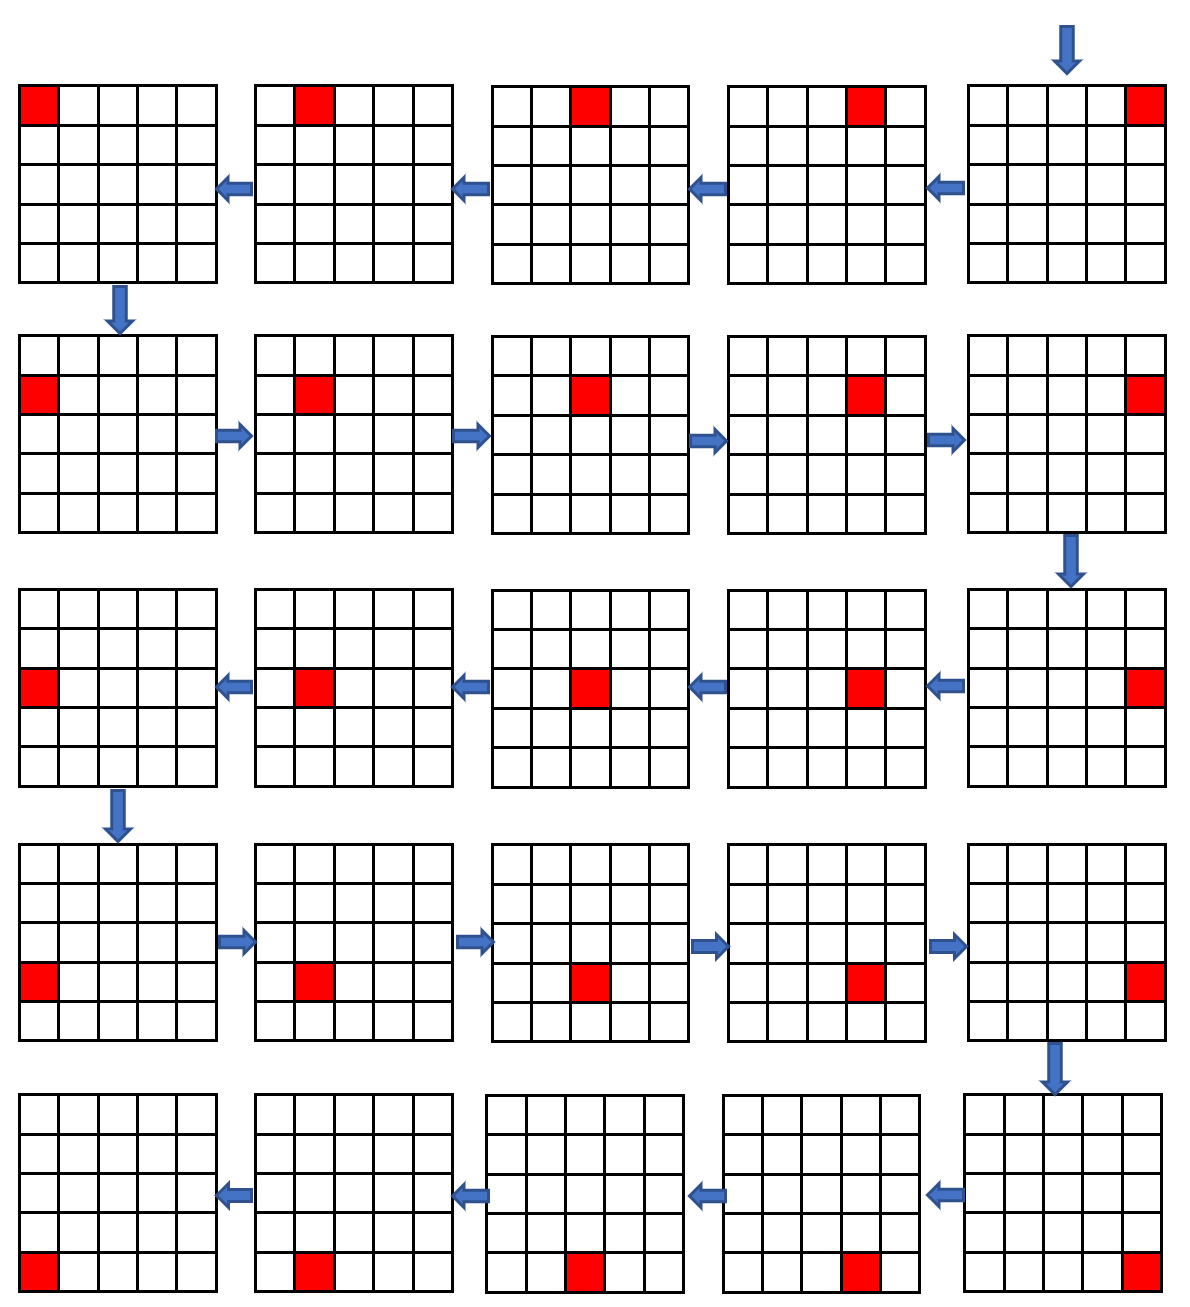
\includegraphics[width=0.6 \linewidth]{figuren/looplicht}
\centering
\caption{De volgorde van het looplicht.}
\label{fig:loopl}
\end{figure}

Begin rechtsboven (bit 0 van de ${0^{e}}$ rij in de matrix) en zet vervolgens steeds de LED links aan. Doe dit tot laatste LED van de rij.
Ga 1 rij naar beneden en zet vervolgens de LED rechts van de rij aan. Doe dit tot en met het $1^{e}$ bit.
Ga 1 rij naar beneden en zet vervolgens de LED links van de rij aan. Doe dit tot en met de laatste LED en ga vervolgens een rij naar beneden.
Doe dit tot en met de laatste rij en begin vervolgens weer op de eerste rij, zoals in het volgende filmpje \href{https://www.youtube.com/shorts/8ZyYWEiXsm0} {
	looplicht}
	te zien is.\\
\textbf{Upload het resultaat op blackboard.}
\end{enumerate}

\paragraph{Challenge opdracht}\label{opdr:accSens}

Op de micro:bit zitten verschillende sensoren. Eén van de sensoren is een \href{https://youtu.be/9WAckt2vrrQ}{accelerometer sensor}.
Het programma in listing \ref{lst:acc} toont de x,y en z waarde van de accelerator sensor.
\begin{enumerate}

	\item Download  listing \ref{lst:acc} van \href{https://github.com/JohnVi-hhs/embsysP/tree/main/voorbeelden/accelerator.ino}{ GitHub} of van brightspace of kopieer listing \ref{lst:acc} in een nieuwe arduino omgeving en voer deze uit.
	\item Pas het programma zodanig aan, zodat de LED in de richting beweegt, waarin micro:kit gehouden wordt.

	\end{enumerate}

\begin{lstlisting}[caption={Looplicht van de bovenste rij.},label={lst:acc}]
#include <LSM303AGR_ACC_Sensor.h>

#define DEV_I2C Wire1   // Wire1 is voor de interne I2C bus 
#define LED ROW1 


// Nodig voor de accelerator 
LSM303AGR_ACC_Sensor Acc(&DEV_I2C);


const int COL1 = 4;   
const int ROW1 = 21;   

void setup() {
	// Led.
	
	pinMode(COL1, OUTPUT);
	digitalWrite(COL1, LOW);
	pinMode(ROW1, OUTPUT);
	
	// Initialisatie van de serieele.
	Serial.begin(9600);
	
	// Initialisate I2C bus (wordt veel gebruikt om sensors).
	DEV_I2C.begin();
	
	// Initialisatie van de accelarator.
	Acc.begin();
	Acc.Enable();
	
	uint8_t a;
	Acc.IO_Read(&a,0x0F,1);
	Serial.print("Ik ben: ");
	Serial.println(a);
}

void loop() {
	// Led blinking.
	digitalWrite(LED, HIGH);
	delay(250);
	digitalWrite(LED, LOW);
	delay(250);
	
	// Lees de accelerometer van de LSM303AGR uit.
	int32_t accelerometer[3];
	Acc.GetAxes(accelerometer);
	
	// Output data.
	Serial.print("| Acc[x/y/z] ");
	Serial.print(accelerometer[0]);
	Serial.print(" ");
	Serial.print(accelerometer[1]);
	Serial.print(" ");
	Serial.print(accelerometer[2]);
	Serial.println(" |");
}
\end{lstlisting}

